\documentclass[10pt,a4paper]{article}

\usepackage[utf8]{inputenc}
\usepackage[LGR,T1]{fontenc}
\usepackage[greek,english]{babel}
\usepackage[english]{isodate}
\usepackage[parfill]{parskip}
\usepackage{graphicx}
\usepackage{pdfpages}
\usepackage{setspace}
\usepackage{amsmath}
\usepackage{listings}
\usepackage{color}
\usepackage{fancyhdr}
\usepackage{hyperref}
\hypersetup{
    colorlinks=true,
    linktoc=all,
    linkcolor=black,
}
\title{%
  \huge \textgreek{Ανάκτηση Πληροφορίας} \\
\large biznasearch - \textgreek{Μηχανή αναζήτησης επιχειρήσεων}}
\author{
    \textgreek{Δημήτριος Ν. Κουβέρης} (2730) \\
    \textgreek{Αλβάρο Α. Χύσι} (2574)
}
\date{\textgreek{Απρίλιος} 2019}

\begin{document}


% cover page
\pagenumbering{gobble}

\maketitle
\newpage

\renewcommand{\contentsname}{\textgreek{Περιεχόμενα}}
\tableofcontents

\pagenumbering{arabic}

% introduction
\newpage
\section{\textgreek{Εισαγωγή}}
\textgreek{
    Η παρούσα εργασία έχει σαν στόχο την κατασκευή μηχανής αναζήτησης
    για δεδομένα επιχειρήσεων. Η μηχανή αναζήτησης υλοποιήθηκε για
    το μάθημα Ανάκτηση Πληροφορίας, τμήμα Μηχανικών Η/Υ και Πληροφορικής,
    Πανεπιστήμιο Ιωαννίνων.
}



\section{\textgreek{Προεπεξεργασία}}
\textgreek{
    Η υλοποίηση έγινε χρησιμοποιώντας δεδομένα επιχειρήσεων απο το
}
Yelp dataset \\ https://www.yelp.com/dataset/challenge

\textgreek{
    Παρακάτω παρουσιάζονται τα βήματα που έγιναν για την προεπεξεργασία
    των δεδομένων.
}

\subsection{\textgreek{Βάση δεδομένων}}
\textgreek{
    Με στόχο την καλύτερη και ευκολότερη διαχείρηση των δεδομένων σε μια
    πιο δομημένη μορφή, δημιουργήθηκε σχεσιακή βάση δεδομένων.

    Το σύστημα διαχείρησης της βάσης δεδομένων που χρησιμοποιήθηκε
    είναι $Postgres$. Το σχήμα που δημιουργήθηκε φαίνεται παρακάτω.

    \begin{center}
        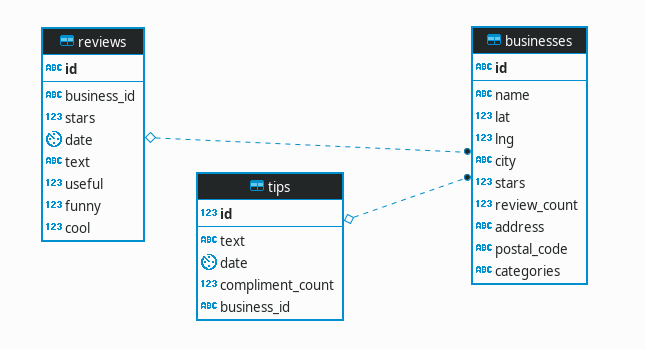
\includegraphics[width=130mm]{media/schema.png}
    \end{center}
}

\subsection{\textgreek{Εισαγωγή δεδομένων}}
\textgreek{
    Η αρχική μορφή των δεδομένων ήταν τύπου $json$.
    Τα δεδομένα μετατράπηκαν
    σε μορφή τύπου $tsv$, με σκοπό την ταχύτερη εισαγωγή τους στη βάση δεδομένων.

    Για τη μετατροπή χρησιμοποιήθηκε το πρόγραμμα $jq$.
    Το $script$ για την
    \\ μετατροπή είναι το $src/main/resources/json\_to\_csv.sh$

    Έπειτα για την εισαγωγή των δεδομένων απο τα $tsv$ αρχεία χρησιμοποιήθηκαν
    εντολές τύπου $COPY$, για παράδειγμα για τον πίνακα των επιχειρήσεων:
} \\
\texttt{COPY businesses FROM '/path/to/businesses.tsv' DELIMITER '\textbackslash t'}

\subsection{\textgreek{Στατιστικά δεδομένων}}
\textgreek{
    Στην παρούσα φάση όλα τα δεδομένα έχουν εισαχθεί στην βάση δεδομένων,
    με κατάλληλα ερωτήματα $SQL$ μπορούμε να βγάλουμε χρήσιμα στατιστικά
    προκειμένου να γίνει καλύτερη κατανόηση των δεδομένων μας.
}

\paragraph{\textgreek{Στατιστικά πόλεων.}}
\textgreek{
    Σε αυτό το βήμα φαίνονται μερικά χρήσιμα στατιστικά ανα πόλη.

    \begin{enumerate}
        \item \textgreek{Αριθμός επιχειρήσεων ανά πόλη.}
        \item \textgreek{Αριθμός κριτικών ανά πόλη.}
        \item \textgreek{Μέσος αριθμός κριτικών και υποδείξεων.}
        \item \textgreek{Αριθμός υποδείξεων ($tips$) ανά πόλη.}
    \end{enumerate}

    \begin{center}
        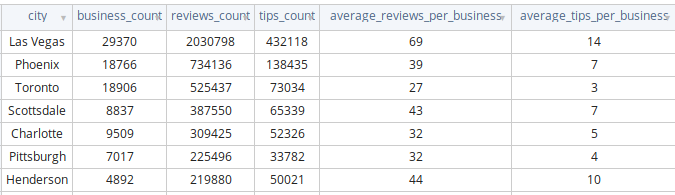
\includegraphics[width=130mm]{media/stats_table.png}
        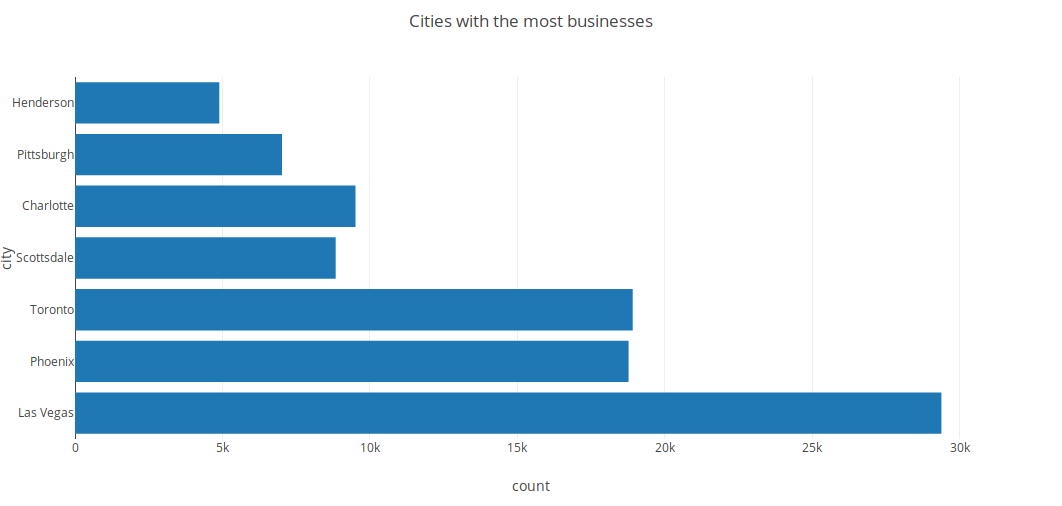
\includegraphics[width=130mm]{media/business_count_chart.png}
        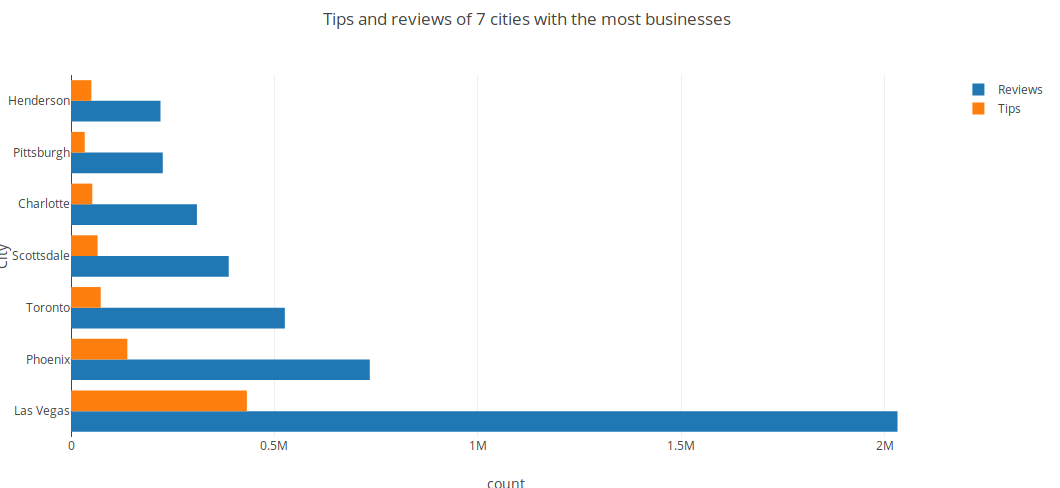
\includegraphics[width=130mm]{media/reviews_and_tips_chart.png}
    \end{center}
}

\paragraph{\textgreek{Στατιστικά επιχειρήσεων.}}
\textgreek{
    Σε αυτό το βήμα παρουσιάζονται μερικά χρήσιμα στατιστικά επιχειρήσεων.

    \begin{enumerate}
        \item \textgreek{Ελάχιστος αριθμός κριτικών και υποδείξεων.}
        
        \item \textgreek{Μέγιστος αριθμός κριτικών και υποδείξεων.}
        \item \textgreek{Μέσος όρος βαθμολογιών.}
        \item \textgreek{Μέσος όρος βαθμολογιών ανά πόλη.}
    \end{enumerate}
}
\paragraph{\textgreek{Η επιλογή μας.}}
\textgreek{
    Σύμφωνα με τα παραπάνω σχήματα, η μηχανή αναζήτησής μας θα αφορά την πόλη του $Las $$Vegas$, αφού είναι η μόνη που
    πληρεί τα κριτήρια της εργασίας, δηλαδή περισσότερες από 10000 επιχειρήσεις και πάνω απο 1000000
    κριτικές και υποδείξεις.
}

\subsection{\textgreek{Φιλτράρισμα}}
\textgreek{
    Σε αυτήν την περίπτωση, μπορούμε να εντοπίσουμε παράγοντες
    θορύβου, όπως για παράδειγμα ανεπιθύμητες ($spam$) κριτικές και υποδείξεις
    καθώς και μη έγκυρες επιχειρήσεις.

    Οι επιχειρήσεις και οι κριτικές που δεν περνάνε κατά το στάδιο του
    φιλτραρίσματος, μένουν στην βάση δεδομένων παρόλα αυτά δεν 
    χρησιμοποιούνται κατά την ευρετηρίαση και άρα δεν εμφανίζονται και 
    δεν λαμβάνονται υπόψιν στα αποτελέσματα.

    \begin{enumerate}
        \item \textgreek{Φιλτράρισμα πόλεων.\\
        Η μηχανή αναζήτησης πρέπει να λαμβάνει υπόψιν επιχειρήσεις μόνο
        μίας πόλης, για τον λόγο αυτό θα χρησιμοποιηθεί η πόλη με τις
        περισσότερες επιχειρήσεις.}
        \item \textgreek{Εντοπισμός ανεπιθύμητων ($spam$) κριτικών και υποδέιξεων.\\
        Ο εντοπισμός γίνεται με βάση τον αριθμό λέξεων, το μήκος λέξεων καθώς και
        την συχνότητα εμφάνισης των λέξεων.}
        \item \textgreek{Εντοπισμός μη έγκυρων επιχειρήσεων.\\
        Μη έγκυρες μπορούν να θεωρηθούν επιχειρήσεις με μη επιτρεπτό όνομα,
        ελλειπή στοιχεία, κτλπ.}
    \end{enumerate}
}

\subsection{\textgreek{Ευρετηρίαση}}

\textgreek{
    Κατά την ευρετηρίαση θα δημιουργηθούν τρία ευρετήρια, ένα για κάθε πίνακα.
}

\paragraph{\textgreek{Επιχειρήσεις}} {
    \textgreek{
        Κάθε επιχείρηση είναι ένα έγγραφο, τα πεδία που χρησιμοποιούνται
        κατά την ευρετηρίαση των επιχειρήσεων, είναι το αναγνωριστικό καθώς
        και το όνομα τους. Το όνομα χρησιμοποιείται κατά την αναζήτηση, ενώ
        το αναγνωριστικό για την ανάκτηση λοιπών πληροφοριών για την επιχείρηση.
    }
}

\paragraph{\textgreek{Κριτικές και υποδείξεις}} {
    \textgreek{
        Κάθε κριτική και υπόδειξη αποτελείται απο ένα έγγραφο. Τα πεδία
        που χρησιμοποιούνται κατά την ευρετηρίαση είναι το αναγνωριστικό 
        της επιχείρησης καθώς και το κείμενο απο το οποίο αποτελούνται.
        Το κείμενο χρησιμοποιείται κατά την αναζήτηση, ενώ το
        αναγνωριστικό για την ανάκτηση λοιπών πληροφοριών για την επιχείρηση.
    }
}



\section{\textgreek{Περιγραφή συστήματος}}
\textgreek{
    Παρακάτω θα περιγράψουμε την διεπαφή του χρήστη καθώς και τον τρόπο
    με τον οποίο θα γίνεται η αναζήτηση.
}

\subsection{\textgreek{Εφαρμογή αναζήτησης}}
\textgreek{
    Για την χρήση του συστήματος απο τελικούς χρήστες θα υλοποιηθεί διαδυκτιακή
    εφαρμογή. Πιο συγκεκριμένα, θα υπάρχει ένας διακομιστής ο οποίος θα δέχεται
    αιτήματα αναζήτησης και θα απαντάει με τα αποτελέσματα σε μορφή
    $json$ έπειτα τα αποτελέσματα θα εμφανίζονται στον φυλλομετρητή του χρήστη.
}

\subsection{\textgreek{Φίλτρα αναζήτησης}}
\textgreek{
    Ο χρήστης θα έχει την δυνατότητα να επιλέξει με βάση ποιό πεδίο θέλει να
    γίνει η αναζήτηση (επιχειρήσεις, κριτικές, υποδείξεις) καθώς και την δυνατότητα
    αναζήτησης χωρίς τον καθορισμό κάποιου πεδίου.

    Κατά την αναζήτηση χωρίς καθορισμό πεδίου το σύστημα θα πρέπει να είναι σε
    θέση να δίνει βαρύτητα στα πεδία και να επιστρέφει τα πιο σχετικά αποτελέσματα.
}

\subsection{\textgreek{Έλεγχος σφαλμάτων}}
\textgreek{
    Το σύστημα επιπλέον θα υποστηρίζει έλεγχο σφαλμάτων καθώς και δυνατότητα
    αυτόματης συμπλήρωσης του ερωτήματος. Έτσι για παράδειγμα εάν ο χρήστης κάνει
    αναζήτηση για επιχειρήσεις με όνομα $Ssame$ τότε το σύστημα θα του προβάλει ερώτηση
    για το έαν εννοούσε $Sesame$.
}

\subsection{\textgreek{Αναδιάταξη αποτελεσμάτων}}
\textgreek{
    Το σύστημα θα υποστηρίζει αναδιάταξη αποτελεσμάτων με βάση τα πεδία της
    επιχείρησης. Αυτό θα γίνεται χρησιμοποιώντας ευρετήριο της βάσης δεδομένων
    στα πεδία που θέλουμε να υποστηρίζουν αναδιάταξη.
}



\section{\textgreek{Μετα-δεδομένα}}
\textgreek{
    Το σύστημα κατα την λειτουργία του θα κρατάει στατιστικά στοιχεία
    απο τις προηγούμενες αναζητήσεις που έχουν γίνει.

    Με βάση τα μετα-δεδομένα το σύστημα θα μπορεί να εμφανίσει τις πιο δημοφιλείς
    επιχειρήσεις, να αναδιατάξει τα αποτελέσματα με βάση τα στατιστικά ερωτήσεων,
    να υποδείξει στους κατόχους των επιχειρήσεων τις πιο σημαντικές λέξεις κλειδιά
    για την επιχείρηση τους και να τους βοηθήσει να βγάλουν χρήσιμα συμπεράσματα για αυτές.
    Τα στατιστικά λειτουργία είναι ιδιαίτερα χρήσιμα για τον έλεγχο λειτουργίας του
    ορθής του συστήματος καθώς και την σύγκριση του με άλλα παρόμοια συστήματα.

    \paragraph{Στατιστικά ερωτήσεων}
    Το σύστημα θα κρατάει στατιστικά για της ερωτήσεις που έχουν γίνει
    καθώς και για τις πιο δημοφιλείς επιχειρήσεις.

    \paragraph{Στατιστικά εμφάνισης}
    Το σύστημα θα κρατάει στατιστικά στοιχεία για τον αριθμό εμφανίσεων
    των επιχειρήσεων στα αποτελέσματα, την θέση της επιχείρησης στα αποτελέσματα
    καθώς και την ερώτηση που την έφερε σε αυτή την θέση.

    \paragraph{Στατιστικά λειτουργίας}
    Το συστημα θα κρατάει πληροφορία για τον χρόνο εξυπηρέτησης τον ερωτημάτων,
    τον αριθμό των αιτημάτων που εξυπηρέτησε, κτλπ...
}


\section{\textgreek{Εφαρμογή}}
\subsection{\textgreek{Γενική περιγραφή}}
\textgreek {
    Η εφαρμογή είναι βασισμένη στην αρχιτεκτονική του $WEB$ και ...
}


\subsection{\textgreek{Περιγραφή $API$}}
\textgreek {
    Στην παρούσα ενότητα θα περιγραφθούν αναλυτικά όλα τα $API$ $endpoints$ που
    υπάρχουν στο σύστημα.

    \texttt {
        \\
        Αίτημα: $GET$ \\
        $URL: /search$ \\
        Περιγραφή: Αναζήτηση επιχειρήσεων \\
        Παράμετροι: \\
        $query$ - Το κείμενο της αναζήτησης \\
        $results-num$ - Ο αριθμός των αποτελεσμάτων \\
        $order-by$ - Το πεδίο της ταξινόμησης
            $("review_count", "-review_count", "stars", "-stars", "clicks", "-clicks", "")$
    }

}


\subsection{\textgreek{Περιγραφή $UI$}}
\input{app-ui.tex}


\end{document}
